\subsubsection{Capas LSTM}\label{lstm_theory}

Las \acrfull{lstm} (Memorias a corto-largo plazo en español), son las capas recurrentes más usadas por su capacidad de mantener dependencias a largo plazo y son usadas extensamente en comunidades de aprendizaje profundo.
\newline

La clave detrás de las \acrshort{lstm} son las puertas que permite a la neurona añadir o eliminar activamente información. Está formado por varias función de activación $\sigma$ y una $tanh$. La función de activación $\sigma$ tiene como consecuencia que el valor de salida sea un valor entre $0$ y $1$. Intuitivamente se puede pensar en que estas funciones tienen como objetivo  capturar y retener información entre $0$, o nada, y $1$, todo.

A continuación se puede ver un diagrama de como funciona una puerta \acrshort{lstm}.


\begin{figure}[H]
    \centering
    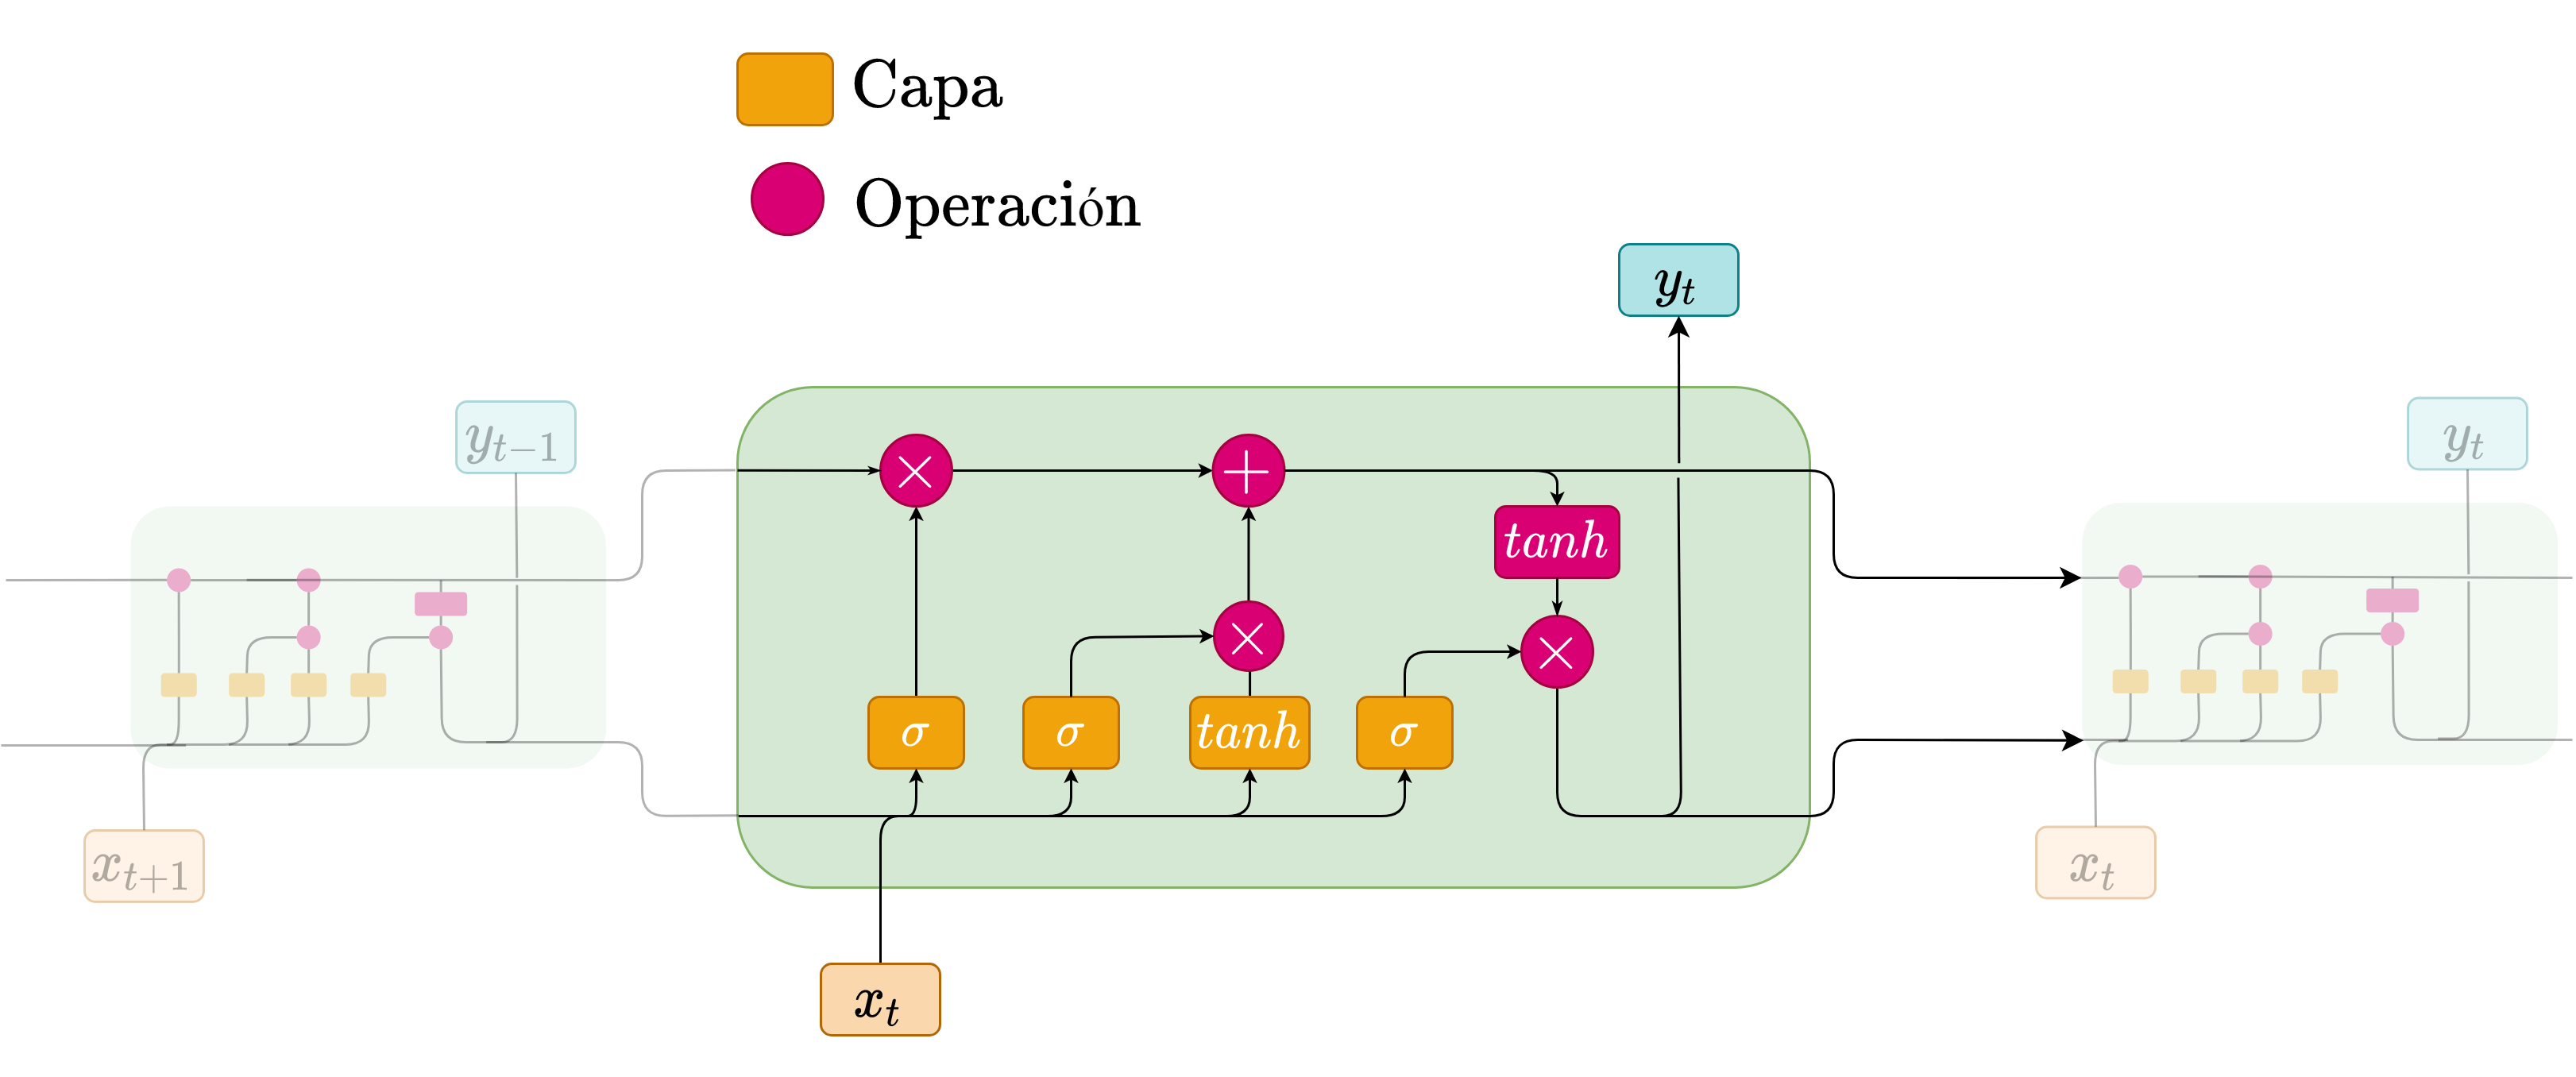
\includegraphics[width=16cm]{images/state-of-art/rnn/lstm.png}
    \caption{Funcionamiento de una \acrshort{lstm}}
\end{figure}


% TODO Añadir ct_1 y ht_1
Las \acrshort{lstm} se forman básicamente por cuatro pasos distintos:
\begin{enumerate}
    \item Olvidar la información irrelevante: En la primera salida de Esta parte es la primera función $\sigma$ junto a la operación del producto escalar entre la salida de $\sigma$ y el estado anterior $h_{t-1}$.
    \item Guardar nueva información: Está formada por la segunda función $\sigma$ y la función $tanh$ al lado suya.
    \item Usar los dos pasos anteriores para calcular un nuevo estado interno $h_t$: Es la parte representada por la línea superior y calcular $c_t$. Suele considerarse a este vector como la memoria de \acrshort{lstm}.
    \item Computar el valor de salida $y_t$: Formada por la última función $\sigma$ y por la función $tanh$. Controla que información es la importante y guarda la información sobre el estado actual.
\end{enumerate}

Con este diseño de puertas se puede diseñar una neurona recursiva que permita el flujo de los gradientes de forma ininterrumpida y evitando su desvanecimiento.
\newline

%TODO LSTM GRADIENT FLWO
% https://youtu.be/SEnXr6v2ifU?list=PLtBw6njQRU-rwp5__7C0oIVt26ZgjG9NI&t=2109
 
 En resumen, una neurona \acrshort{lstm} permite separar en dos partes tanto la memoria como el estado interno permitiendo así que la red pueda aprender dependencias a largo plazo en una secuencia. Esto lo hace mediante el uso de puertas para controlar el flujo de información: olvidando información irrelevante, guardando información importante, actualizando el estado interno de forma selectiva y guardando parte de la información. Todo ello permitiendo que el flujo de los gradiente sea inalterado para evitar el desvanecimiento del gradiente.